\documentclass[12pt]{article}
\usepackage{amsmath} %for underset
\usepackage{bm}
\usepackage[top=1in, bottom=1in, left=1.25in, right=1.25in]{geometry}
\usepackage{cite,bbm}
\usepackage{url}
\usepackage{subfigure}
\usepackage{graphicx}
\usepackage{amssymb}
\usepackage{caption}
\usepackage{multirow}
\usepackage{authblk}
\usepackage{mathtools}
\usepackage{multirow}
\usepackage{fixmath}
\captionsetup{figurewithin=section}
\newcommand\independent{\protect\mathpalette{\protect\independenT}{\perp}}
\def\independenT#1#2{\mathrel{\rlap{$#1#2$}\mkern2mu{#1#2}}}
%\title{Multimodal Deep Learning Library}
%\author[*]{Jian Jin}
%\author[*]{Raman Arora}
%\affil[*]{Department of Computer Science, Johns Hopkins University}
\begin{document}
\title{\vspace{40mm}Multimodal Deep Learning Library}
\author[]{Jian Jin\\{\small Supervised by: Raman Arora}}
\affil{Department of Computer Science, Johns Hopkins University}
\maketitle
\thispagestyle{empty} 

%\begin{flushright}
%Jian Jin\\
%Raman Arora\\
%2015\\
%\end{flushright}
\newpage
\tableofcontents
\newpage

\section{Multimodal Deep Learning Library}
\subsection{Introduction}
This is the document of Multimodal Deep Learning Library, MDL, which is written in C++. It explains principles and implementations with details of Restricted Boltzmann Machine, Deep Neural Network, Deep Belief Network, Denoising Autoencoder, Deep Boltzmann Machine, Deep Canonical Correlation Analysis, and modal prediction model.\\
\\
MDL uses OpenCV 3.0.0, which is the only dependency of this library. Most of its implementation has been tested in Mac OS. It also provides interface for reading various data set such as MNIST, CIFAR, XRMB, and AVLetters. To read mat file, Matlab must be installed because it uses Matlab/c++ interface provided by Matlab.\\
\\
There are multiple model options provided. Different gradient descent methods, loss function, annealing methods, and activation functions are given. These options are easy to extend given the structure of MDL. So MDL could be used as a frame for testings in deep learning.
\subsection{Content Description}
Section 2 goes through common networks. Section 3 to section 7 give descriptions of Restricted Boltzmann Machine, Deep Neural Network, Deep Belief Network, Denoising Autoencoder, Deep Boltzmann Machine, and Deep Canonical Correlation Analysis respectively. Section 8 introduces multimodal learning models. Section 9 gives explanation of the library structure. Section 10 presents performance.\\
\\
In sections 3 to 7, each section explains principles and implementations of each model. Section 8 introduces two models in Multimodal learning.
\clearpage
\section{Network Survey}
This section includes a brief description of network models that are mentioned in this documents and a summary of deep learning models of MDL.
\subsection{Neural Network}
The Neural Network is a directed graph consists of multiple layers of neurons, which is also referred to as units. In general there is no connection between units of the same layer and there are only connections between adjacent layers. The first layer is the input and is referred to as visible layer $v$. Above the visible layer there are multiple hidden layers $\{h_1, h_2,..., h_n\}$. And the output of the last hidden layer forms the output layer $o$.\\
\\
In hidden layers, neurons in layer $h_{i}$ receives input from the previous layer,  $h_{i - 1}$ or $v$, and the output of $h_i$ is the input to the next layer, $h_{i+1}$ or $o$. The value transmitted between layers is called action or emission. Action is computed as:\begin{gather}
a^{(k)}_i = f((\sum_{j=1}^{n_{k-1}}a^{(k-1)}_jw^{k}_{ij})+b^{(k)}_i)=f(z^{(k)}_i)
\end{gather}
where $g$ is the activation function that enables nonlinear representation of the Neural Network. Without activation function the network could only represent linear combination of the input and its power would be much weaker. A common activation function is sigmoid function. $z^{(k)}_i$ is the total input of the unit $i$ in layer $k$. It is computed as a weighted sum of the activations of the previous layer. The weight $w^{k}_{ij}$ and the bias $b^k_i$ is learned in bakcpropagation.\\
\\
A process called forward propagation computes actions layer by layer. Learning of neural network uses backpropagation, which is a supervised learning algorithm. It computes error based on the network output and the training label, then uses this error to compute gradient of error with respect to the weights and biases of each layer, and updates model parameters by gradient descent.
\subsection{Markov Random Field}
A Markov Random Field, also called the Markov Network, is an undirected graphical model in which each node is independent of the other nodes given all the nodes connected to it. It describes the distribution of variables in the graph.\\
\\
The Markov Random Field uses energy to decribe the distribution over the graph\begin{equation}
P(u) = \frac{1}{Z} e^{-E(u)},
\end{equation}
where $Z$ is a partition function defined by \begin{equation}
Z = \sum_{u} e^{-E(u)},
\end{equation}
$E$ is the energy specified by the model, and $u$ is the set of states of all the nodes such that \begin{equation}
u=\{v_1, v_2,...,v_n \}
\end{equation}
where $v_i$ is the state of node $i$.
\subsection{Belief Network}
The Belief Network, which is also referred to as the Bayesian Network, is an directed acyclic graph for probabilistic reasoning. It exhibits the conditional dependencies of the models by associating each node $X$ with a conditional probability $P(X|Pa(X))$ where $Pa(X)$ denotes the parents of $X$. Here are two of its conditional independence property:\\
\\
1. Each node is conditionally independent of its non-descendants given its parents.\\
2. Each node is conditionally independent of all other nodes given its Markov blanket, which consists of its parents, children, and children's parents.\\
\\
The inference of Belief Network is to compute the posterior probability distribution\begin{equation}
P(H|V) = \frac{P(H, V)}{\sum_H P(H,V)}
\end{equation}
where $H$ is the set of query variables that forms hidden units, and $V$ is the set of evidence variables that forms visible units. Approximate inference involves sampling to compute posterior.\\
\\
The Sigmoid Belief Network is a type of the Belief Network such that \begin{equation}
P(X_i=1|Pa(X_i)) = \sigma(\sum_{X_j\in Pa(X_i)} W_{ji} X_j + b_i)
\end{equation}
where $W_{ji}$ is the weight assigned to the edge from $X_j$ to $X_i$. 
\subsection{Deep Learning Models}
The Restricted Boltzmann Machine is a type of Markov Random Field and is trained in an unsupervised manner. It is the building block for other models and could be used for classification by adding a classifier on top of it.\\
\\
The Deep Neural Network is a neural network with multiple layers. Each layer is initialized by pretraing a Restricted Boltzmann Machine. Then fine tuning would refine the parameters of the model.\\
\\
The Deep Belief Network is a hybrid of the Restricted Boltzmann Machine and the Sigmoid Belief Network. It is a generative model, and is not a feedfoward neural network or multilayer perceptron even though its training is similar to the Deep Neural Network.\\
\\
The Denoising Autoencoder is a type of neural network that has symmetric structure. It could reconstruct the input data and if properly trained could reconstruct corrupted images. However, unlike neural networks, It could be trained in an unsupervised manner.\\
\\
The Deep Boltzmann Machine is another type of Markov Random Field. It is pretrained by stacking Restricted Boltzmann Machines with adjusted weights and biases as an approximation to undirected graphs. Its fine tuninig uses a method called mean field inference.\\
\\
The Deep Canonical Correlation Analysis is used for learning multiview or multimodal data by adding a Kernel Canonical Correlation Analysis layer on top of two networks. It finds the projections of the outputs that maximizes their correlation.

\clearpage
\section{Restricted Boltzmann Machine}
\subsection{Logic of Restricted Boltzmann Machine}
\begin{figure}[h]
\centering
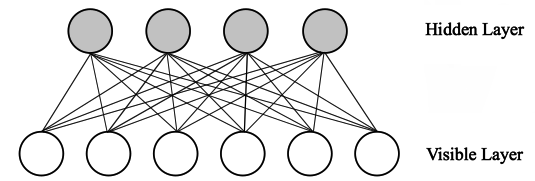
\includegraphics[height=1.5in]{RBM.png}
\caption{Restricted Boltzmann Machine} \label{fig:side:a}
\end{figure}
A Restricted Boltzmann Machine (RBM) is a Markov Random Field consisting of one hidden layer and one visible layer. It is an undirected bipartite graph in which connections are between the hidden layer and the visible layer. Each unit $x$ is a stochastic binary unit such that\begin{equation}
state(x)=\begin{cases}1,~~~~p\\
0,~~~~1-p
\end{cases}
\end{equation}
where probability $p$ is defined by the model. Figure 3.1 shows a RBM with four hidden units and six visible units.\\
\\
As a Markov Random Field, a Restricted Boltzmann Machine defines the  distribution over the visible layer $v$ and the hidden layer $h$ as \begin{equation}
P(v,h) = \frac{1}{Z} e^{-E(v,h)},\label{eq:3}
\end{equation}
where $Z$ is a partition function defined by \begin{equation}
Z = \sum_{v, h} e^{-E(v,h)},
\end{equation}
Its energy $E(v,h)$ is defined by \begin{equation}\label{eq:1}
E(v,h) = -\sum_i b^v_i v_i - \sum_j b^h_j h_j -\sum_i \sum_j v_i w_{i,j} h_j
\end{equation}
where $b^v_i$ is the bias of the \emph{i}th visible unit and $b^h_j$ is the bias of the \emph{j}th hidden unit.\\
\\
Given the conditional independence property of the Markov Random Field, in RBM probability of one layer given the other layer could be factorized as
\begin{gather}
P(h|v)=\prod_j P(h_j|v) \label{eq:2}\\
P(v|h)=\prod_i P(v_i|h).
\end{gather}
Plug equation \eqref{eq:1} in equation \eqref{eq:3}: \begin{equation} \label{eq:5}
P(h|v)=\frac{P(h,v)}{\sum_{h'} P(h',v)}=\frac{exp(\sum_i b^v_i v_i + \sum_j b^h_j h_j +\sum_i \sum_j v_i w_{i,j} h_j)}{\sum_{h'} exp(\sum_i b^v_i v_i + \sum_j b^{h'}_j h'_j +\sum_i \sum_j v_i w_{i,j} h'_j)}.
\end{equation}
And through derivation one could get\begin{equation}\label{eq:4}
\frac{exp(\sum_i b^v_i v_i + \sum_j b^h_j h_j +\sum_i \sum_j v_i w_{i,j} h_j)}{\sum_{h'} exp(\sum_i b^v_i v_i + \sum_j b^{h'}_j h'_j +\sum_i \sum_j v_i w_{i,j} h'_j)}=\prod_{j}\frac{exp(b^h_j + \sum_{i=1}^m W_{i,j} v_i )}{1+exp(b^h_j + \sum_{i=1}^m w_{i,j} v_i )}.
\end{equation}
Combine equation \eqref{eq:2}, \eqref{eq:5}, and \eqref{eq:4} one could get
\begin{equation}
P(h_j=1|v) = \sigma \left(b^h_j + \sum_{i=1}^{N_v} W_{i,j} v_i \right)\,
\end{equation}
where $\sigma$ is a sigmoid function\begin{equation}
\sigma(t) = \frac{1} {1 + exp(-t)}.
\end{equation}
Similarly,
\begin{equation}
P(v_i=1|h) = \sigma \left(b^v_i + \sum_{j=1}^{N_h} W_{i,j} h_j \right).
\end{equation}
\\
A Restricted Boltzmann Machine maximizes the likelihood $P(x)$ of the input data $x$, which is\begin{align}
P(x) = \sum_h P(x,h) = \sum_h \frac{1}{Z}e^{-E(h, x)}=\frac{1}{Z}e^{-F(x)}
\end{align}
where $F(x)$ is called Free Energy such that \begin{equation}
F(x) = - \sum_{i=1}^{n_v} b^v_ix_i-\sum_{j=1}^{n_h}\log(1+ exp(b^h_j+\sum_{k=1}^{n_v} W_{kj}x_k)).
\end{equation}
\\
In training, maximizing the likelihood of the training data is achieved by minimizing the negative log likelihood of the training data. Because the direct solution is intractable, gradient descent is used, in which weights $\{W_{ij}\}$, biases of hidden units $\{b^h_j\}$, and biases of visible units $\{b^v_i\}$ are updated. The gradient is approximated by an algorithm called Contrastive Divergence. More details are in the training section.\\
\\
Express the hidden states $\{h_j\}$ in a row vector $h$, hidden biases $\{b^h_{j}\}$ in a row vector $b^ h$, and weights $\{W_{ij}\}$ in a matrix $W$, which indicates the weight from the visible layer to the hidden layer. The activation of hidden layer is computed as
\begin{equation}
a^h =\sigma(v * W + b^h).
\end{equation}
where $\sigma$ is element-wise performed. Boltzmann Machine acquired tied weights such that
\begin{equation}
a^v = \sigma(h * W^{T} + b^v).
\end{equation}
In training, the state of the visible layer is initialized as training data.
\subsection{Training of Restricted Boltzmann Machine}
In training of Restricted Boltzmann Machine, the weights and the biases of the hidden and the visible layers are updated by gradient descent. Instead of stochastic gradient descent, in which each update is based on each data sample, batch learning is used in RBM training. In batch learning, each update is based on a batch of training data. There are several epochs in training. Each epoch goes through the training data once.\\
\\
For instance if the input data has 10,000 samples and the number of batches is 200, then there will be 200 updates in each epoch.  For each update, gradients will be based on 50 samples. If the number of epochs is 10, commonly there should be a total of 2000 updates in the training process. If the gradients computed are trivial, this process may stop earlier.\\
\\
The gradients of weights are given by Contrastive Divergence as: \begin{equation}\label{eq:7}
\nabla W_{ij} = \langle v_i * h_j\rangle_{recon} - \langle v_i * h_j\rangle_{data}
\end{equation}
where the angle brackets are expectations under the distribution specified by the
subscript. The expectations here are approximated by data sample mean. So it would be 
\begin{equation}
\nabla W_{ij} = \sum_{k = 1} ^ {m}((v_i * h_j)_{recon_k} - (v_i * h_j)_{data_k}) / m
\end{equation}
where $m$ is the size of each data batch.\\
\\
States of the visible layer and hidden layer form a sample in Gibbs sampling, in which  the first sample gives states with the subscript "data" in equation \eqref{eq:7}  and the second sample gives states with the subscript "recon" in equation \eqref{eq:7}. Contrastive Divergence states that one step of Gibbs sampling, which computes the first and the second sample, approximates the descent with high accuracy. In RBM, Gibbs sampling works in the following manner:\\
\\
In Gibbs sampling, each sample $X = (x_1, \dots, x_n)$ is constructed from a joint distribution $\left.p(x_1, \dots, x_n)\right.$ by sampling each component variable from its posterior. Specifically, in the (\emph{i} + 1)th sample $X^{(i+1)} = (x_1^{(i+1)}, \dots, x_n^{(i+1)})$, $x_j^{(i+1)}$ is sampled from \begin{equation}
p(X_j|x_1^{(i+1)},\dots,x_{j-1}^{(i+1)},x_{j+1}^{(i)},\dots,x_n^{(i)}),
\end{equation}
in which the latest sampled component variables are used to compute posterior. Sampling each component variable $x_j$ once forms a sample.\\
\\
Each unit of RBM is a stochastic binary unit and its state is either 0 or 1. To sample $h_j$ from \begin{equation}
P(h_j=1|v) = \sigma \left(b_j + \sum_{i=1}^m W_{i,j} v_i \right),
\end{equation}
simply compute $a_j = \sigma \left(b_j + \sum_{i=1}^m W_{i,j} v_i \right)$. If $a_j$ is larger than a random sample from uniform distribution, state of $h_j$ is 1, otherwise 0. This method works because the probability that a random sample $u$ from uniform distribution is smaller than $a_j$  is $a_j$: \begin{equation}
P(u < a_j) = F_{\text{uniform}}(a_j) = a_j.
\end{equation}
So we have \begin{equation}
P(h_j=1|v) = P(u < a_j).
\end{equation}
Thus we could sample by testing if $u < a_j$, since it has the same probability from which we want to sample. Each unit has two states. If $u < a_j$ fails, the state is 0.\\
\\
In training, first use training data to compute hidden layer posterior using \begin{equation}
P(h_j=1|v) = \sigma \left(b_j + \sum_{i=1}^m W_{i,j} v_i \right).
\end{equation}
The hidden layer states together with the data form the first sample. Then use Gibbs sampling to compute the second sample.\\
\\
The gradient of the visible bias is \begin{equation}
\nabla b^v_{i} = \langle v_i\rangle_{recon} - \langle v_i\rangle_{data},
\end{equation}
and the gradient of the hidden bias is \begin{equation}
\nabla b^h_{j} = \langle h_j\rangle_{recon} - \langle h_j\rangle_{data}
\end{equation}
\subsection{Tricks in Restricted Boltzmann Machine Training}
\textbf{Dropout}\\
Dropout is a method to prevent neural networks from overfitting by randomly blocking emissions from certain neurons. It is similar to adding noise. In RBM training, a mask is generated and put on the hidden layer.\\
\\
For instance, suppose the hidden states are \begin{equation}
h = \{h_1, h_2, ..., h_n\}
\end{equation}
and the dropout rate is $r$. Then a mask $m$ is generated by 
\begin{eqnarray}
m_i=\begin{cases}
1,~~~~u_i > r\\
0,~~~~u_i \leq r
\end{cases}
\end{eqnarray}
where $u_i$ is a sample from uniform distribution, and $i\in \{1, 2, ..., n\}$. The emission of hidden layer would be \begin{equation}
\tilde{h} = h.* m
\end{equation}
where $.*$ denotes element-wise multiplication of two vectors. $\tilde{h}$, instead of $h$, is used to calculate visible states.\\
\\
\textbf{Learning Rate Annealing}\\
There are multiple methods to adapt the learning rate in gradient descent. If the learning rate is trivial, updates may tend to stuck in local minima and waste computation. If it is too large, the updates may bound around minima and could not go deeper. In annealing, learning rate decay helps ensure the learning rate is not too large.\\
\\
Suppose $\alpha$ is the learning rate. In exponential decay, the annealed rate is\begin{equation}
\alpha_a = \alpha * e^{-kt},
\end{equation}
where $t$ is the index of the current epoch, $k$ is a customized coefficient. In divide decay, the annealed rate is\begin{equation}
\alpha_a = \alpha / (1 + kt).
\end{equation}
A more common method is step decay:\begin{equation}
\alpha_a = \alpha * 0.5^{\lfloor{t / 5}\rfloor{}}.
\end{equation}
where learning rate is reduced by half every five epochs. The coefficients in the decay method should be tuned in testings.\\
\\
\textbf{Momentum}\\
With momentum $\rho$, the update step is \begin{equation}
\Delta_{t+1} W = \rho * \Delta_t W - r\nabla W.
\end{equation}
The update value is a portion of previous update value minus the gradient. The intuition behind it is that if the gradient has the same direction as previous update, the update will become larger. If the the gradient is in the different direction from the previous update, the current update will not have the same direction as the gradient and its variance is reduced. In this way, time to converge is reduced.\\
\\
Momentum is often applied with annealing so that steps of updates will not be too large. A feasible scheme is \begin{eqnarray}
\rho=\begin{cases}
0.5,~~~~t <  5\\
0.9,~~~~t \geq 5
\end{cases}
\end{eqnarray}
where $t$ is the index of the current epoch.\\
\\
\textbf{Weight Decay}\\
In weight decay, a penalty term is added to the gradient as a regularizer. $L_1$ penalty $p_1$ is \begin{equation}
p_1 = k \times \sum_{i,j} |W_{ij}|.
\end{equation}
$L_1$ penalty causes many weights to become zero and a few weights to become large. $L_2$ penalty $p_2$ is \begin{equation}
p_2 = k \times \sum_{i,j} W_{ij}^2.
\end{equation}
$L_2$ penalty causes weights to become more even and smaller. The coefficient $k$ is customized, sometimes 0.5 would work. Penalty must be, as well as the gradient, multiplied by the learning rate so that annealing will not change the model trained. 
\subsection{Classifier of Restricted Boltzmann Machine}
A classifier based on RBM could be constructed by training a classifier layer with softmax activation function on top of the hidden layer. Softmax activation function takes a vector $a = \{a_1, a_2,..., a_q\}$ as input, and outputs a vector $c = \{c_1, c_2,..., c_q\}$ with the same dimension, specifically\begin{equation}
c_i = \frac{e^{a_i}}{\sum_{k=1}^q e^{a_k}}.
\end{equation}
\\
Here one-of-$K$ scheme is used to present the class distribution. If there are $K$ classes in the training data, then the label of a sample in class $i$ is expressed as a vector of length $K$ with only the $i$th element as 1, the others as 0. For instance, if the training data has 5 classes, a sample in the forth class has the label\begin{equation*}
\{0,0,0,1,0\}.
\end{equation*}
\\
For a training set with $K$ classes, there should be $K$ neurons in the classifier layer. For each data sample, the sofxmax activation emits a vector of length $K$. The index of the maximum element in this emission is the label. The elements of the  softmax activation sum to 1 and the activation is the prediction distribution:\begin{equation}
c_i = P\{\text{The sample is in class i}\}.
\end{equation}
\\
Softmax activation takes input of dimension $K$ whereas the hidden layer may have dimension of more than 500. So the projection from the hidden layer to the classifier should be learned. If hidden layer has dimension $n_h$ and there are $K$ classes, the weight of this projection should be a matrix of dimension $n_h\times K$.\\
\\
Backpropagation is used to compute this weight. Among several loss functions, cross entropy loss is a good choice for classification using softmax, which is justified by papers comparing various combinations of activation function and loss function. If the label is presented in one-of-$K$ scheme as a vector $t$, and prediction distribution is $c$,  cross entropy loss is \begin{equation}
L = -\sum_{i = 0}^K t_i log(c_i).
\end{equation}
\\
Use chain rule:\begin{equation}
\frac{\partial L}{\partial W_{ij}} = \sum_{p=1}^K \frac{\partial L}{\partial c_p} \frac{\partial c_p}{\partial W_{ij}}
\end{equation}
and \begin{equation}
\frac{\partial c_p}{\partial W_{ij}}= \sum_{q=1}^K \frac{\partial c_p}{\partial z_q} \frac{\partial z_q}{\partial W_{ij}}
\end{equation}
where $c$ is the output of softmax activation and $z$ is its input. That is to say, \begin{equation}
c_i = \frac{exp(z_i)}{\sum_{p=1}^K exp(z_p)}.
\end{equation} Furthermore\begin{equation}
\frac{\partial L}{\partial c_p} = -\frac{t_p}{c_p}
\end{equation}
\begin{equation}
\frac{\partial c_p}{\partial z_q} = \begin{cases}
c_p(1-c_p)~~~~~~\text{if } p = q
\\
-c_p\times c_q~~~~~~~~\text{if } p \neq q
\end{cases}
\end{equation}
\begin{equation}
\frac{\partial z_q}{\partial W_{ij}} = \begin{cases}
a^h_i~~~~~~\text{if } q = j
\\
0~~~~~~~~\text{if } q \neq j
\end{cases}
\end{equation}
where $a^h_i$ is the activation of hidden layer. Based on above equations, for combination of cross entropy loss and softmax activation \begin{equation}
\frac{\partial L}{\partial W_{ij}} = a_i^h(c_j - t_j)
\end{equation}
Expressed in row vectors it is \begin{equation}
\nabla W = (a^h)^T\times (c - t)
\end{equation}
where $(a^h)^T$ is the transpose of row vector $a^h$. This gradient is used in batch learning.
\subsection{Implementation of RBM}
My implementation of RBM is in the header file rbm.hpp. The RBM class stores information of one hidden layer and one activation layer. It has methods to train a learning or classifier layer. Here is a selected list of methods of class rbm:\\
\\
I. void \textbf{dropout}(double i)\\
-Set dropout rate as input i.\\
\\
II. void \textbf{doubleTrain}(dataInBatch $\&$trainingSet, int numEpoch, int inLayer, ActivationType at = sigmoid$\_$t, LossType lt = MSE, GDType gd = SGD, int numGibbs = 1)\\
-Train an RBM layer in Deep Boltzmann Machine, which is an undirected graph. This part will be explained in DBM section.\\
\\
III. void \textbf{singleTrainBinary}(dataInBatch $\&$trainingSet, int numEpoch, ActivationType at = sigmoid$\_$t, LossType lt = MSE, GDType gd = SGD, int numGibbs = 1);\\
-Train an RBM layer with binary units in Deep Belief Networks and RBM.\\
\\
IV. void \textbf{singleTrainLinear}(dataInBatch $\&$trainingSet, int numEpoch, ActivationType at= sigmoid$\_$t, LossType lt = MSE, GDType gd = SGD, int numGibbs = 1);\\
-Train an RBM layer with linear units.\\
\\
V. void \textbf{singleClassifie}r(dataInBatch $\&$modelOut, dataInBatch $\&$labelSet, int numEpoch, GDType gd = SGD);\\
-Build a classifier layer for RBM.\\
\\
The model could be tested by running runRBM.cpp. First train a RBM with one hidden layer:\\
\\
RBM rbm(784, 500, 0);\\
rbm.dropout(0.2);\\
rbm.singleTrainBinary(trainingData, 6);\\
dataInBatch modelOut = rbm.g$\_$activation(trainingData);\\
\\
The hidden layer has 500 units, and the index of this RBM is 0, which is used for multi-layer model. Then set the dropout rate as 0.2 and train it with 6 epochs. After training, stack another RBM layer with softmax activation function:\\
\\
RBM classifier(500, 10, 0);\\
classifier.singleClassifier(modelOut, trainingLabel, 6);\\
classificationError e = classifyRBM(rbm, classifier, testingData, testingLabel, sigmoid$\_$t);\\
\\
MNIST dataset has 10 classes, so the classifier is of dimension 10.
\subsection{Summary}
RBM is the foundation for several multi-layer models. It is crucial that this component is correctly implemented and fully understood. The classifier may be trained with the hidden layer at the same time. Separating these two facilitates checking problems in the implementation.
\clearpage
\section{Deep Neural Network}
\subsection{Construction of Deep Neural Network}
\begin{figure}[h]
\centering
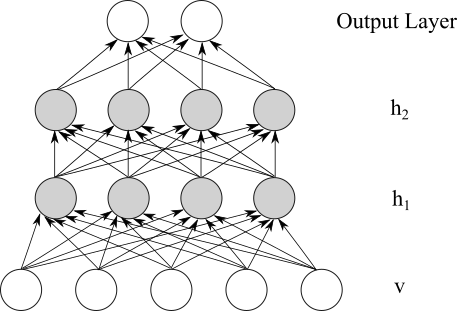
\includegraphics[height=3.2in]{DNN.png}
\caption{Deep Neural Network} \label{fig:side:a}
\end{figure}
A Deep Neural Network (DNN) is a neural network with multiple hidden layers. In neural networks, initialization of weights could greatly effect the training results. Pretraining, in which multiple Restricted Boltzmann Machines are trained to initialize parameters of each DNN layer, provides weight initialization that saves training time. Backpropagation is a time-consuming process. With pretraining, the time consumed by bakckpropagation could be significantly reduced. Figure 4.1 shows a DNN with two hidden layers.\\
\\
Below shows construction of a Deep Neural Network for classification:\\
\\
I. Set the architecture of the model, specifically the size of the visible layer and the hidden layers, \(n_0, n_1, n_2, ..., n_N\). $n_0$ is the input dimension and input forms a visible layer. $n_N$ equals to the number of classes in training data.\\
\\
II. Pretrain hidden layers:\\
for $i = 1\text{ to }N $:\\
\indent 1. Train an RBM with the following settings:\\
\begin{gather*}
n_h^{(i)}=n_i\\
n_v^{(i)}=n_{i-1}\\
d_i=a_{i-1}\\
\end{gather*}
\indent where
\begin{gather*}
n_h^{(i)} = \text{Dimension of hidden layer of RBM trained for layer }i,\\
n_v^{(i)} = \text{Dimension of visible layer of RBM trained for layer }i,\\
d_i = \text{Input of RBM trained for layer i},\\
a_{i-1} = \text{Activations of the }(i-1)\text{th DNN layer}.
\end{gather*}
\indent 2. Set \begin{gather*}
W_i = W_{RBM},\\
b_i = b^h_{RBM},\\
a_i = a_{RBM}.
\end{gather*}
\indent RBM is used to initialize weights and biases of each DNN layer.\\
end for.\\
\\
III. Fine Tuning:\\
Use backpropagation to refine weights and biases of each layer. In backpropagation, one epoch goes through training data once. A dozen of epochs may suffice.\\
\\
Classification with Deep Neural Network is similar to RBM. The last layer, which uses softmax activation, gives the prediction distribution.
\subsection{Fine Tuning of Deep Neural Network}
As mentioned in the above section, fine tuning uses backpropagation, which is a common learning algorithm used in neural networks. Unlike one-step backpropagation used in training classifier of RBM, this one is a thorough one going through each layer. Backprogation algorithm is:\\
\\
I. Perform a pass through all layers of the network, computing total input of each unit $\{z^{(1)},..., z^{(N)}\}$ and activations $\{a^{(1)},..., a^{(N)}\}$ of each layer. $a^{(i)}$ is the row vector that presents the activation of layer $i$. \\
\\
II. For the last layer, compute $\delta_i^{(N)}$ as
\begin{equation}
\delta_i^{(N)} = \frac{\partial L}{\partial z^{(N)}_i}
\end{equation}
where $L$ is the classification error. Acquire a row vector $\delta^{(N)}$. \\
\\
III. For $l$ = $N-1, ...,1$, compute 
\begin{align}
\delta^{(l)} = \left(\delta ~ (W^{(l)})^T \right) \bullet g'(z^{(l)})
\end{align}
where $g$ is the activation function.\\
\\
IV. Compute the gradients in each layer. For $l$ = $N, ..., 1$, compute 
\begin{align}
\nabla_{W^{(l)}} L &= (a^{(l-1)})^T~\delta^{(l)}, \\
\nabla_{b^{(l)}} L &= \delta^{(l)}.
\end{align}
where $a^{(0)}$ is the training data.\\
\\
V. Update the weights and biases of each layer using gradient descent.\\
\\
In fine tuning, the training data should be used repeatedly to refine the model parameters.
\subsection{Implementation of Deep Neural Network}
The implementation of Deep Neural Network is in the header file dnn.hpp. It uses class RBMlayer to store architecture information. Here is a selected list of methods of class dnn:\\
\\
I. void \textbf{addLayer}(RBMlayer $\&$l)\\
Add a layer to the current model. This object of class RBMlayer should store information of layer size, weight, bias, etc. It could also be modified after added to  the model.\\
\\
II. void \textbf{setLayer}(std::vector$<$size$\_$t$>$ rbmSize)\\
Object of class dnn could automatically initialize random weights and biases of each layer by inputting a vector of layer sizes.\\
\\
III. void \textbf{train}(dataInBatch $\&$trainingData, size$\_$t rbmEpoch, LossType l = MSE, ActivationType a = sigmoid$\_$t)\\
This method trains all the layers without classifier. The structure of dnn should be initialized before calling this method. \\
\\
IV. void \textbf{classifier}(dataInBatch $\&$trainingData, dataInBatch $\&$trainingLabel, size$\_$t rbmEpoch, int preTrainOpt, LossType l = MSE, ActivationType a = sigmoid$\_$t)\\
Build a Deep Neural Network with a classifier layer. This function contains pretraining option preTrainOpt. If preTrainOpt=1, pretrain each layer by training RBMs, else randomly initialize layer parameters without pretraining.\\
\\
V. void \textbf{fineTuning}(dataInBatch $\&$label, dataInBatch $\&$inputSet, LossType l)\\
Fine tuning step that uses backpropagation.\\
\\
VI. classificationError \textbf{classify}(dataInBatch $\&$testingSet, dataInBatch $\&$testinglabel);\\
Perform Classification. The result is stored in the format classficationError.
\subsection{Summary}
Construction of the Deep Neural Network is stacking multiple RBMs in the pretraining process and then performing fine tuning. Because the Deep Neural Network is a directed graph and each layer receives input from the previous adjacent layer, there is no extra inference in training this model.
\clearpage
\section{Deep Belief Network}
\subsection{Logic of Deep Belief Network}
\begin{figure}[h]
\centering
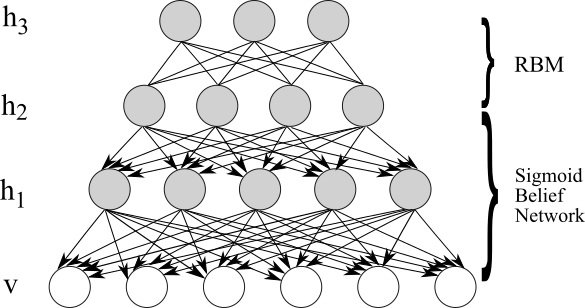
\includegraphics[height=2.8in]{DBN.png}
\caption{Deep Belief Network} \label{fig:side:a}
\end{figure}
A Deep Belief Network (DBN) is a hybrid of a Restricted Boltzmann Machine and a Sigmoid Belief Network. A Deep Belief Network maximizes the likelihood $P(x)$ of the input $x$. Figure 5.1 shows a DBN.\\
\\
For a Deep Belief Network with $N$ hidden layers, the distribution over the visible layer (input data) and hidden layers is\begin{equation}
P(v, h_1, ..., h_N)  = P(v| h_1) \times\left(\prod_{k=1}^{N-2}  P(h_k| h_{k+1}))\right)\times P(h_{N-1},h_N).
\end{equation}
To prove this, express the distribution with chain rule:\begin{equation}
P(v, h_1, ..., h_N)  = P(v| h_1, ..., h_N) \times\left(\prod_{k=1}^{N-2}  P(h_k| h_{k+1},..., h_{N}))\right)\times P(h_{N-1},h_N).
\end{equation}
And in the belief network, each node is independent of its ancestors given its parent. So these hold:\begin{gather}
P(v| h_1, ..., h_N) = P(v|h_1),\\
P(h_k| h_{k+1},..., h_{N}) = P(h_k| h_{k+1}).
\end{gather}
So we have \begin{equation}
P(v, h_1, ..., h_N)  = P(v| h_1) \times\left(\prod_{k=1}^{N-2}  P(h_k| h_{k+1}))\right)\times P(h_{N-1},h_N),
\end{equation}
where $P(v| h_1) \times\left(\prod_{k=1}^{N-2}  P(h_k| h_{k+1}))\right)$ is the distribution over the Sigmoid Belief Network and $P(h_{N-1},h_N)$ is the distribution over Restricted Boltzmann Machine.\\
\\
For classification there should be a layer $y$ on top of the last hidden layer. With  layer $y$ that represents prediction distribution, the distribution over the Deep Belief Network is
\begin{equation}
P(v, h_1, ..., h_N, y)  = P(v| h_1) \times\left(\prod_{k=1}^{N-2}  P(h_k| h_{k+1}))\right)\times P(h_{N-1},h_N, y).
\end{equation}
where $P(h_{N-1},h_N, y)$ could be regarded as the distribution over a RBM which has labels $y$ and the state $h_{N-1}$ as the input.\\
\\
In pretraining of the Deep Belief Network, pretrained RBMs are stacked like in pretraining the Deep Neural Network. However, since this is not a feedforward neural network. A different fine tuning method called Up-Down algorithm is used.
\subsection{Training of Deep Belief Network}
Training a Deep Belief Network is to construct model that maximizes the likelihood of the training data. With the concavity of the logarithm function, the lower bound of the log likelihood of the training data $x$ could be found:\begin{equation}\label{eq:10}
\log P(x)=\log\left(\sum_h Q(h|x)\frac{P(x,h)}{Q(h|x)}\right)\geq \sum_h Q(h|x)\log\frac{P(x,h)}{Q(h|x)}
\end{equation}
and we have
\begin{equation}\label{eq:8}
\sum_h Q(h|x)\log\frac{P(x,h)}{Q(h|x)}= \sum_h Q(h|x)\log P(x, h)-\sum_h Q(h|x)\log Q(h|x)
\end{equation}
where $Q(h|x)$ is an approximation to the true probability $P(h|x)$ of the model.\\
\\
If $Q(h|x) = P(h|x)$, plug it in the right-hand side of \eqref{eq:8} we have \begin{equation}\label{eq:11}
\begin{split}
&\sum_h P(h|x)(\log P(h|x) + \log P(x))-\sum_h P(h|x)\log P(h|x)\\
& = \sum_h P(h|x)\log P(x) =\log P(x)\sum_h P(h|x) =\log P(x).
\end{split}
\end{equation}
Combine equation \eqref{eq:11}, \eqref{eq:8}  with \eqref{eq:10}, we could find that when $Q(h|x) = P(h|x)$, the lower bound is tight.\\
\\
Moreover, the more different $Q(h|x)$ is from $P(h|x)$, the less tight the bound is. The lower bound of \eqref{eq:10} could be expressed as \begin{equation}
\log P(x) - KL(Q(h|x)||P(h|x)).
\end{equation}
Less difference between the approximation $Q(h|x)$ and the true posterior $P(h|x)$ gives lower value of their KL divergence, thus higher bound. Unlike true posterior, the approximations could be factorized\begin{equation}
Q(h|x)=\prod_{i=1}^{n_h} Q(h_i|x).
\end{equation}
\\
Consequently, in training the goal is to find approximation $Q(h|x)$ with high accuracy   and at the same time maximizes the bound. This could be done by stacking pretrained RBMs. The lower bound of \eqref{eq:10} could be factorized as
\begin{equation}\label{eq:9}
\sum_h Q(h|x)\log\frac{P(x,h)}{Q(h|x)}= \sum_h Q(h|x)(\log P(x|h) + \log P(h))-\sum_h Q(h|x)\log Q(h|x)
\end{equation}
In the right-hand side of equation \eqref{eq:9}, $Q(h|x)$ and $P(x|h)$ are given by the first pretrained RBM. So to maximize the lower bound is to maximize \begin{equation}
\sum_h Q(h|x)\log P(h).
\end{equation}
A RBM maximizes the likelihood of the input data. So staking another pretrained RBM on top of the first hidden layer would maximize the lower bound. Moreover, \begin{equation}
P(h) = \sum_{h^{(2)}}P(h, h^{(2)}), 
\end{equation}
where $h^{(2)}$ is computed by the second pretrained RBM. The second RBM takes sample constructed from $Q(h|x)$ as input. But it could be trained independently since its parameters do not depend on the parameters of the first pretrained RBM. This is why greedy layer-wise pretraining works.\\
\\
After pretraining is done, use Up-Down algorithm as fine tuning, which is a combination of the training process of RBM, and an algorithm called Wake-Sleep algorithm which is for learning of the Sigmoid Belief Network.
\subsection{Classification of Deep Belief Network}
In training the Restricted Boltzmann Machine, dropout is used to alleviate overfitting. This method reminds us that RBM has the ability to predict missing values.\\
\\
In a trained deep belief network, each approximation $Q(h_{k+1}|h_k)$ could be computed based on states $h_k$ and model parameters. In a deep belief network with classifier, the top RBM takes labels and hidden layer $h_{N-1}$ to compute states of the last hidden layer $h_N$, which is illustrated in Figure 5.2. For better prediction performance, when training the top RBM, dropout is used.\\
\\
Suppose $l$ is the set of units that represent prediction distribution. In classification, fill $l$ with zeros and compute approximation $Q(h_N|l, h_{N-1})$. Then use the states $h_N$ sampled from $Q(h_N|l, h_{N-1})$ to compute prediction distribution $l$ by $P(l, h_{N-1}| h_N)$.
\begin{figure}[h]
\centering
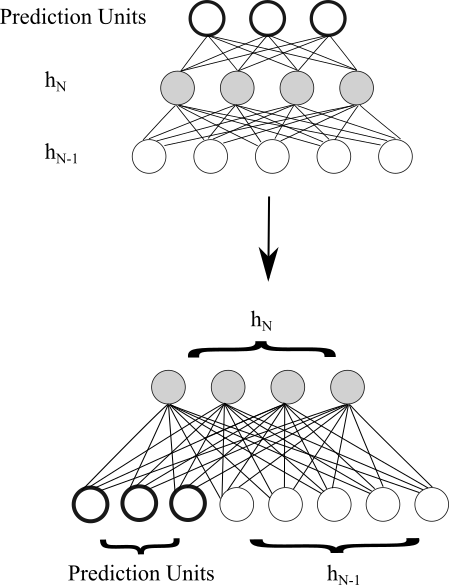
\includegraphics[height=5.0in]{DBNclass.png}
\caption{Top RBM of DBN with classifier} \label{fig:side:a}
\end{figure}
\subsection{Implementation of Deep Belief Network}
The implementation of Deep Belief Network is in the header file dbn.hpp. It uses class RBMlayer to store architecture information. Here is a selected list of methods of class dnn:\\
\\
I. void \textbf{addLayer}(RBMlayer $\&$l)\\
Add a layer to the current model. This object of class RBMlayer should store information of layer size, weight, bias, etc. It could also be modified after added to  the model.\\
\\
II. void \textbf{setLayer}(std::vector$<$size$\_$t$>$ rbmSize)\\
Object of class dnn could automatically initialize random weights and biases of each layer by inputting a vector of layer sizes.\\
\\
III. void \textbf{train}(dataInBatch $\&$trainingData, size$\_$t rbmEpoch, LossType l = MSE, ActivationType a = sigmoid$\_$t)\\
This method trains a dbn without classifier. The architecture of dbn should be initialized before calling this method. \\
\\
IV. void \textbf{classifier}(dataInBatch $\&$trainingData, dataInBatch $\&$trainingLabel, size$\_$t rbmEpoch, LossType l = MSE, ActivationType a = sigmoid$\_$t)\\
This method trains a dbn with classifier. The architecture of dbn should be initialized before calling this method.\\
\\
V. void \textbf{fineTuning}(dataInBatch $\&$dataSet, dataInBatch $\&$labelSet, int epoch)\\
The fine tuning uses Up-Down algorithm.\\
\\
VI. classificationError \textbf{classify}(dataInBatch $\&$testingSet, dataInBatch $\&$testinglabel);\\
Perform Classification.
\subsection{Summary}
It is easy to confuse the Deep Belief Network with the Deep Neural Network. Both of them stack pretrained RBMs in the training process. However, because these two models have distinct structures, their classification processes are different. In the Deep Neural Network, forward propagation gives the prediction distribution whereas in the Deep Belief Network the prediction distribution is computed by one more projection from the last hidden layer. They also use different fine tuning methods.
\clearpage
\section{Denoising Autoencoder}
\subsection{Construction of Autoencoder}
\begin{figure}[h]
\centering
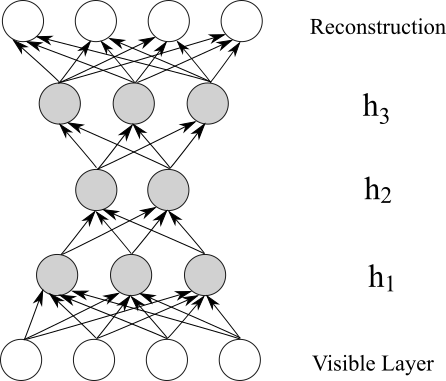
\includegraphics[height=3.2in]{AE.png}
\caption{Autoencoder} \label{fig:side:a}
\end{figure}
Autoencoder(AE) is a type of neural network forming  a directed graph. Its symmetricity states that for an autoencoder with $(N + 1)$ layers (including visible layer and output layer), the dimension of each layer is constrained by \begin{gather}
n_i = n_{N - i}~~~~\text{for }0\leq i\leq N
\end{gather}
where $n_i$ is the dimension of the $i$th layer, and $n_0$ is the input dimension. Since the output layer and the visible layer are in the same dimension, it is expected that autoencoders could reconstruct the input data. Thus the training of autoencoders is unsupervised learning because input data is used as labels in fine tuning, and reconstruction errors could be used to access the model. Autoencoders could also be used to construct classifiers by adding a classifier layer on top of it. Figure 6.1 shows an Autoencoder.\\
\\
Below is how to construct an autoencoder:\\
I. Set the architecture of the model, specifically the size of each layer, \(n_0, n_1, n_2, ..., n_N\).\\
\\
II. Pretraining:\\
for $i = 1\text{ to }N/2$:\\
\indent 1. Train an RBM with the following settings:\\
\begin{gather*}
n_h^{(i)}=n_i\\
n_v^{(i)}=n_{i-1}\\
d_i=a_{i-1}
\end{gather*}
\indent where
\begin{gather*}
n_h^{(i)} = \text{Dimension of hidden layer of RBM trained for layer }i,\\
n_v^{(i)} = \text{Dimension of visible layer of RBM trained for layer }i,\\
d_i = \text{Input of RBM trained for layer i},\\
a_{i-1} = \text{Activations of the }(i-1)\text{th layer of autoencoder},
\end{gather*}
\indent 2. Initialize parameters of the current layer
\begin{gather*}
W_i = W_{RBM},\\
b_i = b^h_{RBM},\\
a_i = a_{RBM}.
\end{gather*}
\indent The parameters of trained RBM are used to initialize the parameters of the layer.\\
end for.\\
\\
for $i = N/2+1\text{ to }N$:\\
\indent Initialize paramers \begin{gather*}
W_i = W_{N - i}^{T},\\
b_i = b_{N-i}.
\end{gather*}
end for.\\
\\
III. Fine Tuning:\\
Backpropagation with Mean Square Error. Error is computed based on the reconstruction and the training data.
\subsection{Fine tuning of Autoencoder}
Fine tuning of Autoencoder uses backpropagation, which is:\\
\\
I. Perform a forward propagation through all layers that computes layer inputs $\{z^{(1)},..., z^{(N)}\}$ and activations $\{a^{(1)},..., a^{(N)}\}$. $a^{(i)}$ is a row vector representing the activation of layer $i$. \\
\\
II. For the last layer, compute $\delta_i^{(N)}$ as
\begin{equation}
\delta_i^{(N)} = \frac{\partial L}{\partial z^{(N)}_i}
\end{equation}
where $L$ is the reconstruction error. This step acquires a row vector $\delta^{(N)}$. \\
\\
III. For $l$ = $N-1, ..., 1$, compute 
\begin{align}
\delta^{(l)} = \left(\delta^{(l+1)} ~ (W^{(l)})^T \right) \bullet g'(z^{(l)})
\end{align}
where $g$ is the activation function and here $g'$ is element-wise performed.\\
\\
IV. Compute the gradients in each layer. For $l$ = $N, ..., 1$, compute 
\begin{align}
\nabla_{W^{(l)}} L &= (a^{(l-1)})^T~\delta^{(l)}, \\
\nabla_{b^{(l)}} L &= \delta^{(l)}.
\end{align}
where $a^{(0)}$ is the input data of the autoencoder.\\
\\
V. Update the weights and biases of each layer with gradient descent.\\
\\
The reconstruction error of Autoencodr is \begin{equation}
L = \frac{1}{2}\sum_{i=1}^{n_N}(a^{(N)}_i - a^{(0)}_i)^2
\end{equation}
where \begin{gather*}
n_{N} = \text{Dimension of the output/reconstruction},\\
a^{(N)}_{i} = \text{Activation of the }i\text{th unit in the output layer},\\
a^{(0)}_{i} = \text{Activation of the }i\text{th unit in the visible layer}.
\end{gather*}
Backpropagation involves computing $\{\delta^{(i)}\}$, which is based on the derivatives of activation function and error function. Here is how to compute these two values:\\
\\
For sigmoid activation:
\begin{equation}
g'(t) = \frac{\partial{(1+e^{-t})^{-1}}}{\partial{t}} = \frac{1}{1+e^{-t}}\frac{e^{-t}}{1+e^{-t}}.
\end{equation}
That is to say\begin{equation}
g'(z_i) = \frac{1}{1+e^{-z_i}}(1-\frac{1}{1+e^{-z_i}})=a_i(1-a_i).
\end{equation}
For $\delta_i^{(N)}$, use chain rule\begin{equation}
\delta_i^{(N)} = \frac{\partial L}{\partial z^{(N)}_i}=\sum_{p=1}^{n_N} \frac{\partial L}{\partial a^{(N)}_p} \frac{\partial a^{(N)}_p}{\partial z^{(N)}_i} = \frac{\partial L}{\partial a^{(N)}_i} \frac{\partial a^{(N)}_i}{\partial z^{(N)}_i} = (a^{(N)}_i-a^{(0)}_i)\times a^{(N)}_i(1-a^{(N)}_i).
\end{equation}
\subsection{Denoising Autoencoder}
The Denoising Autoencoder reconstructs the input from its corrupted version. So it could predict missing values and it is quite straightforward to observe its performance when the input is image data. By putting a denoise mask on the input, the Autoencoders could be transformed to the Denoising Autoencoders. Here is how to make this transformation:\\
\\
Firstly a denoise rate $r$ is chosen, and the mask is constructed as follows:\begin{equation}
m_i=\begin{cases} 
1,~~~~\text{if }U_i > r\\
0,~~~~\text{otherwise}\\
\end{cases}
~~1\leq i\leq n_N\\
\end{equation}
where $U_i$ is the $i$th sample from uniform distribution, $n_N$ is the size of the last layer, which is also the dimension of input data.\\
\\
Secondly compute the corrupted input data\begin{equation}
a^{(c)} = a^{(0)}\cdot m = \sum_{i=1}^{n_N} a^{(0)}_im_i
\end{equation}\\
\\
Finally use $a^{(c)}$ as the training data to compute the reconstruction and still use the uncorrupted data $a^{(0)}$ as labels in fine tuning.\\
\\
Fine tuning in the Denoising Autoencoder makes more improvement in reconstruction than in the Autoencoder, and is crucial in the Denoising Autoencoder.
\subsection{Implementation of Denoising Autoencoder}
The implementation of DAE is in the header file autoencoder.hpp.\\
\\
I. void \textbf{addLayer}(RBMlayer $\&$l)\\
Add a layer to current DAE. This object of class RBMlayer should store information of layer size, weight, bias, etc. It could also be modified after added to DAE.\\
\\
II. void \textbf{setLayer}(std::vector$<$size$\_$t$>$ rbmSize)\\
Object of class AutoEncoder could automatically initialize random weights and biases of each layer by inputting a vector of layer sizes.\\
\\
III. void \textbf{train}(dataInBatch $\&$trainingData, size$\_$t rbmEpoch, LossType l = MSE, ActivationType a = sigmoid$\_$t)\\
This method trains all the layers without classifier. The structure of this AutoEncoder object should be initialized before calling this method. \\
\\
IV. void \textbf{reconstruct}(dataInBatch $\&$testingData)\\
Give the reconstruction of the testingData and stores the result in the model. This method should be called only after the model has been trained.\\
\\
V. dataInBatch \textbf{g$\_$reconstruction}()\\
Get the reconstruction.\\
\\
VI. void \textbf{fineTuning}(dataInBatch $\&$originSet, dataInBatch $\&$inputSet, LossType l)\\
Use backpropagation. Unlike DBN, argument LossType should be MSE instead of CrossEntropy.\\
\\
VI. void \textbf{denoise}(double dr)\\
Set the denoise rate as dr. When model is in training, it will detect if denoise rate is set. So if this method is called before training, the Denoising Autoencoder will be trained automatically. Otherwise the Autoencoder will be trained.
\subsection{Summary}
Construction of the Denoising Autoencoder requires pretraining half of its layers, the other half is set by its symmetric structure. Fine tuninig is crucial for Denoising Autoencoder because it uses uncorrupted data to modify the model trained with corrupted data. The performance of Denoising Autoencoder is straightforward to assess because one could observe the reconstructed images.
\clearpage
\section{Deep Boltzmann Machine}
\subsection{Logic of Deep Boltzmann Machine}
\begin{figure}[h]
\centering
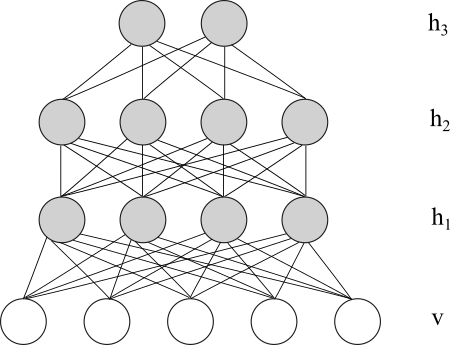
\includegraphics[height=2.8in]{DBM.png}
\caption{Deep Boltzmann Machine} \label{fig:side:a}
\end{figure}
A Deep Boltzmann Machine(DBM) is a Markov Random Field consisting of multiple layers. Connections exist only between adjacent layers. Intuitively, it could incorporate top-down feedback when computing bottom-up approximations. Figure 7.1 shows a DBM.\\
\\
The energy function of a Deep Boltzmann Machine with $N$ hidden layers is\begin{equation}
E(v, h^{(1)},..h^{(N)})=-v^{T}W^{(1)}h^{(1)} -(h^{(1)})^TW^{(2)}h^{(2)}-...- (h^{(N-1)})^TW^{(N)}h^{(N)}
\end{equation}
where $W^{(i)}$ is the weight from the previous layer to the $i$th hidden layer.\\
\\
A Deep Boltzmann Machine maximizes the likelihood of the input data. The gradient of its log likelihood is \begin{equation}
\frac{\partial \log P(v)}{\partial W^{(i)}} = \langle h^{(i-1)}(h^{(i)})^T\rangle_{data} - \langle h^{(i-1)}(h^{(i)})^T\rangle_{model}.
\end{equation}
\subsection{Pretraining of Deep Boltzmann Machine}
Because the Deep Boltzmann Machine is an undirected model, the last hidden layer receives input from the previous adjacent layer, and the other hidden layers receive inputs from both directions. So when training Restricted Boltzmann Machines, the weights and biases need to be adjusted for better approximations. The pretraining process is as below:\\
\\
I. Set the architecture of the model, specifically the size of each layer, \(n_0, n_1, n_2, ..., n_N\). $n_0$ is the dimension of the training data.\\
\\
II. Pretrain the first hidden layer:\\
Train an RBM, in which the weight from the visible layer $v$ to the hidden layer $h_1$ is $2W_1$ and the weight from $h_1$ to $v$ is $W_1^{T}$. $W_1$ is the weight of the first DBM hidden layer.\\
\\
III. Pretrain intermediate hidden layers:\\
for $i = 2\text{ to }N - 1$:\\
\indent 1. Train an RBM with the following settings:\\
\begin{gather*}
n_h^{(i)}=n_i\\
n_v^{(i)}=n_{i-1}\\
d_i=a_{i-1}\\
\end{gather*}
\indent where
\begin{gather*}
n_h^{(i)} = \text{Dimension of hidden layer of RBM trained for layer }i,\\
n_v^{(i)} = \text{Dimension of visible layer of RBM trained for layer }i,\\
d_i = \text{Input of RBM trained for layer i},\\
a_{i-1} = \text{Activations of the }(i-1)\text{th layer}.
\end{gather*}
\indent 2. Set \begin{gather*}
W_i = W_{RBM} / 2,\\
b_i = b^h_{RBM} / 2,\\
a_i = a_{RBM}.
\end{gather*}
\indent Weights and biases are adjusted here for better approximations.\\
\\
IV. Pretrain the last hidden layer:\\
Train an RBM, in which the weight from the hidden layer $h_{N-1}$ to the hidden layer $h_N$ is $W_N$ and the weight from $h_{N}$ to $h_{N-1}$ is $2W_N^{T}$. $W_N$ is the weight of the last hidden layer of DBM.
\subsection{Mean Field Inference}
The mean field inference of the Deep Boltzmann Machine involves iterative updates of the approximations $Q$. It is performed after pretraining. The algorithm is as below:\\
\\
\noindent \textbf{Algorithm} Mean Field Inference\\
Initialize $M$ samples $\{\tilde{v}_{0,1},\tilde{h}_{0,1}\}$,...,$\{\tilde{v}_{0,M},\tilde{h}_{0,M}\}$with the pretrained model. Each sample consists of states of the visible layer and all the hidden layers.\\
\noindent \textbf{for} $t = 0$ to $T$ (number of iterations) \textbf{do}\\
\indent 1. \textbf{Variational Inference:}\\
\indent \textbf{for} each data sample \textbf{v}$_n,n=1$ to $D$ \textbf{do}\\
\indent\indent Perform a bottom-up pass with 
\begin{gather*}
\nu_j^1 = \sigma\Big( \sum_{i=1}^{n_0} 2W_{ij}^1v_i \Big),\\
\nu_k^2 = \sigma\Big( \sum_{j=1}^{n_1} 2W_{jk}^2\nu_j^1\Big),\\
\cdots\\
\nu_p^{N-1} = \sigma\Big( \sum_{l=1}^{n_{N-2}} 2W_{lp}^{N-1}\nu_l^{N-2} \Big),\\
\nu_q^{N} = \sigma\Big( \sum_{p=1}^{n_{N-1}} W_{pq}^{N}\nu_p^{N-1} \Big),
\end{gather*}
\indent\indent where $\{W_{ij}\}$ is the set of pretrained weights.\\
\indent\indent Set $\mathbold{\mu}=\mathbold{\nu}$ and run the mean-field updates with:
\begin{gather*}
\mu_j^1 \leftarrow \sigma\Big(\sum_{i=1}^{n_0} W_{ij}^1v_i + \sum_{k=1}^{n_2}W_{jk}^2\mu_k^2 \Big),\\
\cdots\\
\mu_j^{N-1} \leftarrow \sigma\Big(\sum_{i=1}^{n_{N-2}} W_{ij}^{N-1}\mu_i^{N-2} + \sum_{k=1}^{n_N}W_{jk}^N\mu_k^N \Big),\\
\mu_j^{N} \leftarrow \sigma\Big(\sum_{i=1}^{n_{N-1}} W_{ij}^{N}\mu_i^{N-1} \Big).
\end{gather*}
\indent\indent Set $\mathbold{\mu}_n = \mathbold{\mu}$. \par
\textbf{end for}\\
\\
\indent 2. \textbf{Stochastic Approximation:}\\
\indent \textbf{for} each sample $m=1$ to $M$ \textbf{do}\par
\indent\indent Running one step Gibbs sampling. Get $(\tilde{v}_{t+1,m},\tilde{h}_{t+1,m})$ from $(\tilde{v}_{t,m},\tilde{h}_{t,m})$\\
\textbf{end for}\\
\\
\indent 3. Parameter Update:\\
\indent $W^1_{t+1} = W^1_t + \alpha_t\Big(\frac{1}{D}\sum_{n=1}^D \mathbf{v}_n(\mathbold{\mu}_n^1)^T- \frac{1}{M}\sum_{m=1}^M \tilde{\mathbf{v}}_{t+1,m}(\tilde{\mathbf{h}}_{t+1,m}^1)^T\Big)$\\
\indent $W^2_{t+1} = W^2_t + \alpha_t\Big(\frac{1}{D}\sum_{n=1}^D \mathbold{\mu}_n^1(\mathbold{\mu}_n^2)^T- \frac{1}{M}\sum_{m=1}^M \tilde{\mathbf{h}}_{t+1,m}^1(\tilde{\mathbf{h}}_{t+1,m}^2)^T\Big)$\\
\indent $W^3_{t+1} = W^3_t + \alpha_t\Big(\frac{1}{D}\sum_{n=1}^D \mathbold{\mu}_n^2(\mathbold{\mu}_n^3)^T- \frac{1}{M}\sum_{m=1}^M \tilde{\mathbf{h}}_{t+1,m}^2(\tilde{\mathbf{h}}_{t+1,m}^3)^T\Big)$\\
\indent Decrease $\alpha_t$.\\
\noindent \textbf{end for}\\
\\
To facilitate computation, $M$ may be chosen as the number of batches.\\
\subsection{Implementation of Deep Boltzmann Machine}
The implementation of DBM is in the header file dbm.hpp.\\
\\
I. void \textbf{addLayer}(RBMlayer $\&$l)\\
Add a layer to current DBM. This object of class RBMlayer should store information of layer size, weight, bias, etc. It could also be modified after added to DBM.\\
\\
II. void \textbf{setLayer}(std::vector$<$size$\_$t$>$ rbmSize)\\
Object of class DBM could automatically initialize random weights and biases of each layer by inputting a vector of layer sizes.\\
\\
III. void \textbf{train}(dataInBatch $\&$Data, dataInBatch $\&$label, size$\_$t rbmEpoch, LossType l = MSE, ActivationType a = sigmoid$\_$t)\\
This method trains DBM as classifier.\\
\\
IV. void \textbf{fineTuning}(dataInBatch $\&$data, dataInBatch $\&$label)\\
Fine tuning uses mean field inference.\\
\\
V. void \textbf{classify}(dataInBatch $\&$data, dataInBatch $\&$label)\\
Classify the data with DBM. Label set is used to compute classification error rate.
\subsection{Summary}
In DBM, each layer receives input from all its adjacent layers. Its training is more complicated than other models in directed graphs.
\clearpage
\section{Multimodal Learning Model}
\subsection{Deep Canonical Correlation Analysis}
\subsubsection{Canonical Correlation Analysis}
Canonical Correlation Analysis is a method to find the relationship between two sets of variables. Specifically, suppose for two sets of variables $X$ and $Y$, in which each column consists of samples of a variable, there are two projections\begin{gather}
U=a^TX,\\
V=b^TY.
\end{gather}
The correlation between $U$ and $V$ is\begin{equation}
corr(U,V)=\frac{Cov(U,V)}{\sqrt{var(U)var(V)}}.
\end{equation}
The goal is to find the projections $a$ and $b$ that maximize this correlation. To ensure a unique solution, two conditions are added to the goal\begin{gather}
Var(U)=1,\\
Var(V)=1.
\end{gather}
Centering the data will not change the result but could facilitate computation:\begin{gather}
x=X-I_XI_X^TX/n_X,\\
y=Y-I_YI_Y^TY/n_Y.
\end{gather}
where $I_X$ is an $n_X \times 1$ vector of ones, $n_X$ is the number of rows of $X$, and $n_Y$ is the number of rows of $Y$. And the covariance matrix of centered data $x$ is \begin{equation}
Cov(x,x) = Var(x)=x^Tx/(n_x - 1).
\end{equation}
The solution to this problem suggests that $a$ and $b$ are respectively the eigenvectors of the following matrices\begin{gather}
Cov(x,x) ^{-1} Cov(x,y) Cov(y, y) ^{-1} Cov(y, x),\\
Cov(y,y) ^{-1} Cov(y,x) Cov(x, x) ^{-1} Cov(x, y).
\end{gather}
The $i$th eigenvectors of each matrix form the projections weights giving the $i$th largest correlation, and its corresponding eigenvalue is the square of its correlation value.\\
\\
In computing, one could add each column of $y$ to $x$ and form a matrix $m = [x~ y]$. Then \begin{equation}
Var(m) = \left[\begin{array}{ccc}
    Cov(x,x) & Cov(x,y) \\
    Cov(y,x) & Cov(y,y)\\ 
  \end{array}
  \right].
\end{equation}
\subsubsection{Kernel Canonical Correlation Analysis}
Kernel Canonical Correlation Analysis projects the data into a higher-dimensional
feature space before linear projections using the mapping \begin{equation}
\phi\colon x \rightarrow \phi(x).
\end{equation}
In computation, kernel $K(x, y)$ is used, which is defined as\begin{equation}
K(x,y) = \langle \phi (x), \phi (y)\rangle
\end{equation}
where $\langle a, b\rangle$ indicates inner product of $a$ and $b$. The solution suggests that projection $a$ is the top eigenvectos of the matrix\begin{equation}
(K(X,X) + r_XI_XI_X^T)^{-1} K(Y,Y)  (K(Y,Y) + r_YI_YI_Y^T)^{-1} K(X,X),
\end{equation}
where $r_X$ and $r_Y$ are regularized terms.  And $b$ is given by \begin{equation}
b = \frac{1}{\lambda}(K(Y,Y) + r_YI_YI_Y^T)^{-1} K(X,X) a
\end{equation}
where $\lambda$ is the corresponding eigenvalue of $a$. 
\subsubsection{Deep Correlation Analysis}
In Deep Correlation Analysis (DCCA), A layer of KCCA is added on top of two separately trained Deep Neural Networks, of which each learns the data of one modal. Figure 8.1 shows a example of DCCA. With KCCA on the top, the model could learn the correlation between data of two modals.
\begin{figure}[h]
\centering
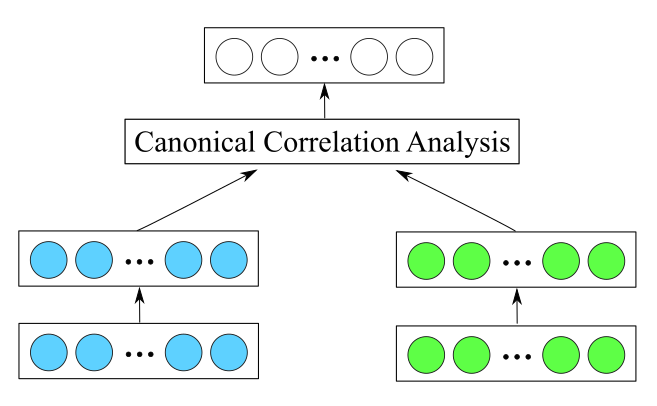
\includegraphics[height=2.8in]{DCCA.png}
\caption{Deep Canonical Correlation Analysis} \label{fig:side:a}
\end{figure}
\subsection{Modal Prediction and Transformation}
\begin{figure*}[!t]
\centering
\subfigure[Bimodal Deep Belief Network] {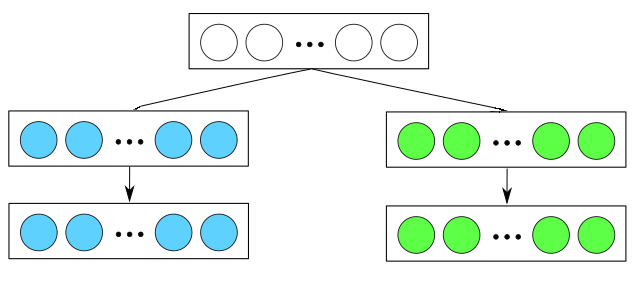
\includegraphics[height=1.2in]{modalPrediction1.png}}
\subfigure[Modal Reconstruction Network] {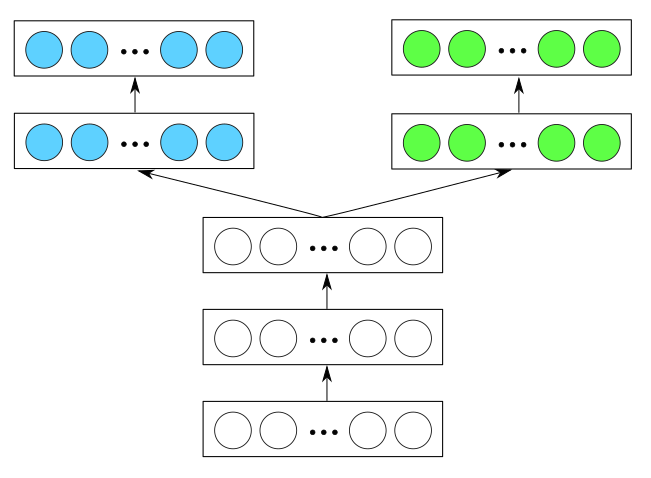
\includegraphics[height=1.8in]{modalPrediction2.png}}
\caption{Modal Prediction}
\label{fig5}
\end{figure*}
\begin{figure}[h]
\centering
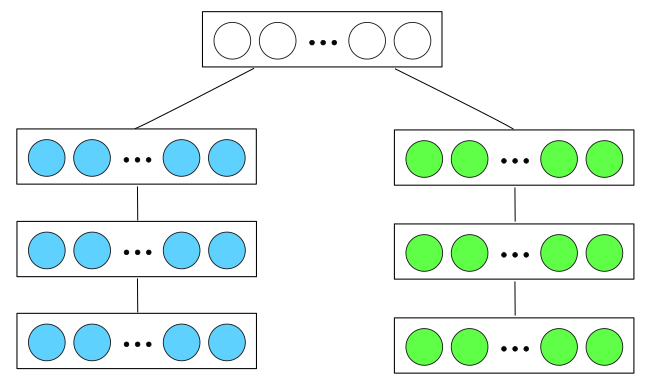
\includegraphics[height=2.2in]{DBMmodals.png}
\caption{MRF Multimodal Learning Model} \label{fig:side:a}
\end{figure}
It is possible to make lower-dimension representation of two modals by building a Bimodal Deep Belief Network as in Figure 8.2(a), in which blue nodes represent data from one modal and green nodes represent data from the other modal. In this process the recognition weights which are used in bottom-up computation and the generative weights which are used in top-down computation should be learned. If the model is trained with tied weights, half of the memory space could be saved since transpose of weight matrix would transform recognition weights to generative weights. The weights of this model could be used to reconstruct data of two modals as in Figure 8.2(b).\\
\\
Another option is to build a Markov Random Field multimodal learning model by combining two Deep Boltzmann Machines. Figure 8.3 shows such a model. This model is constructed by first build two DBMs, each is trained on data of one modal. Then Train an RBM on top of these two DBMs.\\
\\
Prediction of data from one modal given data from the other modal could be done by first training a Bimodal Autoencoder in Figure 8.4(a) and then use the modal prediction network in Figure(b) to predict data from two modals. It would be necessary to add noise to corrupt data when training the Bimodal Autoencoder so that it has more power in reconstruction.
 \begin{figure*}[!t]
\centering
\subfigure[Bimodal Autoencoder] {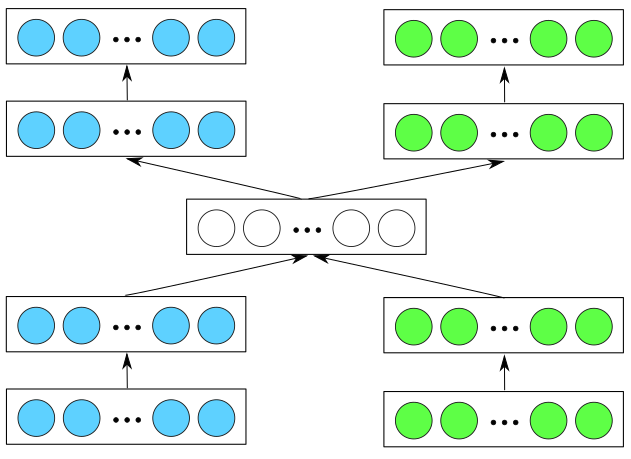
\includegraphics[height=1.8in]{aemodal.png}}
\subfigure[Modal Prediction Network] {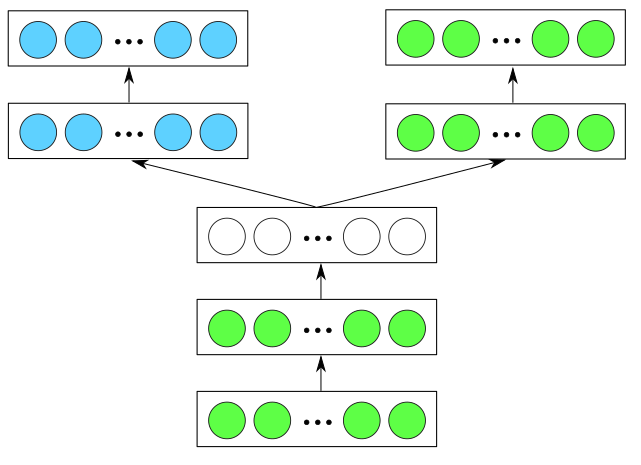
\includegraphics[height=1.8in]{prediction.png}}
\caption{Modal Prediction}
\label{fig5}
\end{figure*}
\clearpage
\section{Library Structure}
\subsection{Data Reading}
\subsubsection{MNIST}
MNIST is a selected set of samples from NIST data set. It has one training data set, one training label set, one testing data set, and one testing label set. The training set has 60,000 samples and the testing set has 10,000 samples. Each sample data is a 28$\times$28 grey image which is a handwritten integer between 0 and 9. It has 10 classes, so the label is between 0 (inclusive) and 9 (inclusive).\\
\\
The data is stored in big-endian format. The content of data should be read as unsigned characters. Header file readMNIST.hpp provides functions to read this data set.\\
\\
I. cv::Mat \textbf{imread$\_$mnist$\_$image}(const char* path)\\
Read data of MNIST. Each row is a sample.\\
\\
II. cv::Mat \textbf{imread$\_$mnist$\_$label}(const char* path)\\
Read labels of MNIST. Each row is a number indicating class of that sample.
\subsubsection{CIFAR}
The CIFAR-10 data set consists of 60000 32x32 colour images in 10 classes, with 6000 images per class. There are 5 batches of training images and 1 batch of test images, each consists of 10000 images.\\
\\
In CIFAR-10 data set, each sample consists of a number indicating its class and the values of the image pixels. Put five training data batches and one testing data batch of CIFAR-10 in the same folder named "data". The following function in the header file readCIFAR.hpp reads them to four OpenCV matrices:\\
\\
void \textbf{imread$\_$cifar}(Mat $\&$trainingData, Mat $\&$trainingLabel, Mat $\&$testingData, Mat $\&$testingLabel)\\
\\
Each row of the read OpenCV matrices consists of the label and the data of a sample.

\subsubsection{XRMB}
As stated in its explanation, Wisconsin X-ray Microbeam Database (XRMB) data used in "Deep Canonical Correlation Analysis" is processed by Galen Andrew, Raman Arora, etc.The dimension of the MFCC data is 273 and the dimension of the XRMB data is 112. There are label files of fold 0 that provides the phone labels. The data is stored in double-precision format.\\
\\
The following function in the header file readXRMB.hpp reads them:\\
\\
cv::Mat \textbf{imread$\_$XRMB$\_$data}(const char* path, int inputDim)\\
\\
indexLabel \textbf{imread$\_$XRMB$\_$label}(const char* path)\\
\\
When reading MFCC files, inputDim = 273. When reading XRMB files, inputDim = 112. The label is between 0 (inclusive) and 39 (inclusive). The data is stored sample by sample. 
\subsubsection{AvLetters}
AvLetters is the data set recording audio data and video data of different people uttering letters. The dimension of the audio data is 26 and the dimension of the video data is 60$\times$80. The data is stored in single-precision big-endian format. Each file is the data of a person uttering a certain letter. For instance, the file A1$\_$Anya.mfcc contains the audio data of the person named Anya uttering letter "A". \\
\\
The following function in the header file readAvLetters.hpp reads audio data:\\
\\
cv::Mat \textbf{imread$\_$avletters$\_$mfcc}(const char* path)\\
\\
The output is an OpenCV matrix, of which each row contains data of a sample. The original video data is in MATLAB file format. The header file readMat.hpp contains the function\\
\\
cv::Mat \textbf{matRead}(const char* fileName, const char* variableName, const char* saveName).\\
\\
It reads the mat file and at the same time saves it as binary file named as the argument "saveName". This header file uses the MATLAB/c++ interface provided by MATLAB and requires an environment setting, which is contained as comments in the header file. There are some problems running the libraries in this interface together with OpenCV. So use this function to transform all MATLAB files to binary files before training models and then read the transformed binary files. The header file readDat.hpp provide the function to read the transformed binary files:\\
\\
cv::Mat \textbf{readBinary}(const char* file, int rowSize, int colSize)\\
\\
The output is an OpenCV matrix, of which each row contains data of a sample.
\subsubsection{Data Processing}
Header file processData.hpp stores functions processing data.\\
\\
data \textbf{oneOfK}(indexLabel l, int labelDim)\\
Transfer index label to one-of-k expression.\\
\\
dataInBatch \textbf{corruptImage}(dataInBatch input, double denoiseRate)\\
Give corrupted data in batches.\\
\\
std::vector$<$dataInBatch$>$ \textbf{dataProcess}(dataCollection$\&$ reading, int numBatch)\\
Build data batches.\\
\\
dataCollection \textbf{shuffleByRow}(dataCollection$\&$ m)\\
Shuffle the data\\
\\
cv::Mat \textbf{denoiseMask}(size$\_$t rowSize, size$\_$t colSize, double rate)\\
Generate a mask to corrupt data
\subsection{Computation and Utilities}
\textbf{activation.hpp} includes multiple activation functions, such as sigmoid, tanh, relu, leaky$\_$relu, softmax. Each activation function is paired with a function that computes its derivatives to facilitate computation in backpropagation.\\
\\
\textbf{cca.hpp} includes functions computing CCA and KCCA.\\
\\
\textbf{gd.hpp} includes functions for adaptive gradient descent and stochastic gradient descent, and a function to anneal the learning rate in which three types of annealing methods are provided.\\
\\
\textbf{inference.hpp} includes the mean field inference implementation used by DBM.\\
\\
\textbf{kernel.hpp} includes multiple kernel functions used by KCCA.\\
\\
\textbf{loss.hpp} includes computation of loss functions. MSE, absolute loss, cross entropy, and binary loss are provided together with the functions to compute their derivatives.\\
\\
\textbf{matrix.hpp} includes some OpenCV matrix manipulation functions.\\
\\
\textbf{loadData.hpp} contains functions to test data loading by visualization.\\
\\
\textbf{visualization.hpp} contains functions of visualization.\\
\subsection{Models and Running}
Table 1 shows the header files and files that contains main functions to test each model. Besides these, modalPrediction.cpp contains implementation of a modal prediction model.
\begin{table}[h]
\centering
\begin{tabular}{|c|c|c|c|c|c|c|}
\hline
Model & RBM & DNN & DBN & DAE/AE & DBM & DCCA\\
\hline
Header(.hpp) & rbm &dnn & dbn & autoencoder & dbm & cca\\
\hline
Main(.cpp) & runRBM & runDNN & runDBN & runDAE &runDBM & runDCCA \\
\hline
\end{tabular}
\caption{Header files of models}
\end{table}
\clearpage
\section{Performance}
\subsection{Restricted Boltzmann Machine}
The main function to run Restricted Boltzmann Machine is in runRBM.cpp. It uses RBM for classification of MNIST data set. On MNIST, use 60,000 samples for training and 10,000 samples for testing. With hidden layer of size 500. The classification error rate is 0.0707 (Accuracy 92.93$\%$). Multiple deep learning libraries give similar results.
\subsection{Deep Neural Network}
The main function to run Deep Neural Network is in runDNN.cpp. Usually it takes a large number of epochs in backpropagation in training. However this number is greatly reduced by pretraining.\\
\\
For testing, a DNN with hidden layers of size 500, 300, 200 respectively is constructed. On MNIST data set, pretraining alone would gives out the error rate of 0.093 (Accuracy 90.7$\%$). In backpropagation, each epoch goes through once the whole training data for update. One epoch in backpropagation gives out classification error rate of 0.0858 (Accuracy 91.42$\%$). Ten epochs in backpropagation gives out classification error rate of 0.0288 (Accuracy 97.12$\%$). Learning rate is 0.01 in fine tuning. The result is similar to the performance of running DNN on MNIST with MEDAL. 
\subsection{Denoising Autoencoder}
The main function to run Denoisinig Autoencoder is in runDAE.cpp. For testing, a Denoising Autoencoder with hidden layers of size 500, 300, 500 is constructed. Figure 10.1 shows the Denoising Autoencoder reconstruction of the corrupted testing set using model trained by training set, in which upper six lines are reconstructions and the lower six lines are uncorrupted input. As a comparison, Figure 10.2 shows the Autoencoder reconstruction of the uncorrupted testing set. Fine tuninig in the Denoising Autoencoder gives more improvement of performance than in the Autoencoder.\\
\\
Each epoch goes through once the whole training data for update. On MNIST, run 10 epochs in fine tuning, the reconstruction error computed by MSE in the Denoising Autoencoder are: Average error without fine tuning 6686.69. Average error after fine tuning 3256.34. The reconstruction error computed by MSE in the Autoencoder are: Average error without fine tuning 4463.24. Average error after fine tuning 3182.69.\\
\\
So after sufficient fine tuning, the reconstruction of Denoising Autoencoder is similar to the reconstruction from the uncorrupted images. The reconstruction visualization is comparable to published result.\\
\begin{figure*}[!t]
\centering
\subfigure[Denoising Autoencoder] {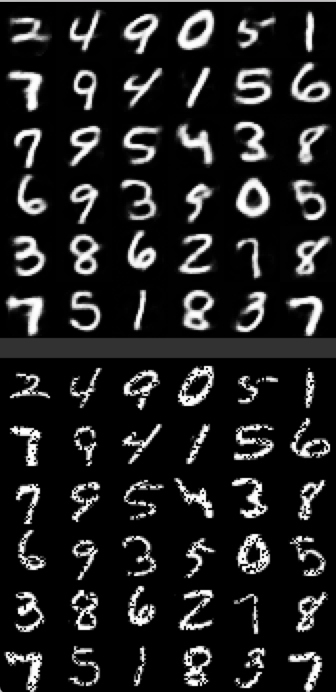
\includegraphics[height=3.5in]{ae3.png}}
\subfigure[Autoencoder] {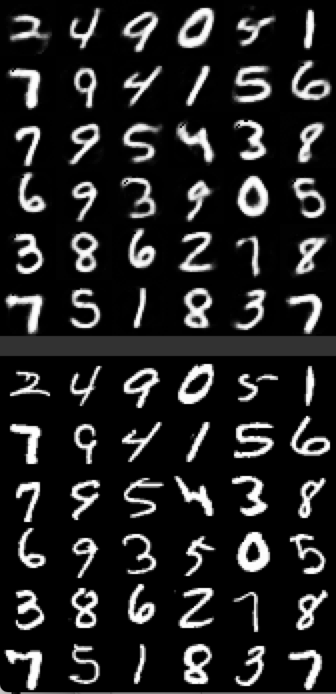
\includegraphics[height=3.5in]{ae2.png}}
\caption{Reconstruction of DAE and AE on MNIST}
\label{fig5}
\end{figure*}

\begin{figure}[h]
\centering
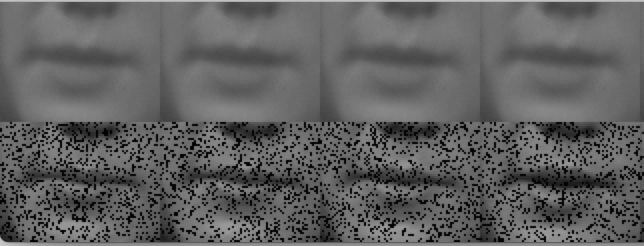
\includegraphics[height=1.3in]{avletterRec.png}
\caption{Denoising Avletter audio data} \label{fig:side:a}
\end{figure}
Another test is made with AvLetters data set, which is in runDAE$\_$letter.cpp. Figure 10.2 shows denosing avletter audio data. It uses the audio data of a person pronouncing "A", "B", "C", "D", "E", "F", "G" to train the model and reconstructs the data of person pronouncing "H" and "I".
\subsection{Deep Belief Network}
The main function to run the Deep Belief Network is in runDBN.cpp. For testing, a Deep Belief Network with hidden layers of sizes 500, 300 is constructed. The classification error rate on MNIST without fine tuning is 0.0883 (Accuracy 91.17$\%$). With the Up-down fine tuning method the classification error rate could be reduced to 0.0695 (Accuracy 93.05$\%$). [6] indicates the best performance of DBN on MNIST could achieve the error rate of 1.25$\%$. There are multiple parameters in the training process could affect the result, such as learning rate and tricks in gradient descent. This possibly affect the result.
\subsection{Deep Boltzmann Machine}
The main function to run the Deep Boltzmann Machine is in runDBM.cpp. For testing, a Deep Boltzmann Machine with hidden layers of sizes 500, 500 is constructed. The error rate on MNIST without fine tuning is 0.0937 (Accuracy 90.63$\%$). Mean Field inference improves the accuracy to 93.47$\%$. Again multiple parameters could affect the result. [5] indicates that the accuracy on MNIST could achieve test error of 0.95$\%$. Its source code uses Conjugate Gradient optimization, which is not implemented in this library. This possibly causes the difference.
\subsection{Deep Canonical Correlation Analysis}
The main function to run DCCA is in runDCCA.cpp. The testing data set is CIFAR-10. Each image is divided as the left and the right halves as data from two views. Then two networks trained on two views are built. Each view of data is of dimension 512. Each network gives the output of dimension 20. The DCCA could quickly find the solution in which the sum of the top 20 correlations is 10.8756. Without network below CCA layer, the solution could not be computed in a reasonable time.\\
\\
A test on AvLetters was also done. Unfortunately the correlation given is close to 0. This suggests that there is very week linear dependence between data of two modals. So it should be another form of dependence existing.
\subsection{Modal Prediction}
Modal prediction implementation is in the modal$\_$prediction.cpp. It trains the modal using audio and video data of uttering letter from "A" to "G" and then uses the audio data of letter "H" and "I" to predict the video data of "H" and "I". The reconstruction error is 10.46$\%$.
\clearpage
%Bibliographic references
\addcontentsline{toc}{section}{References}
\nocite{*}
\bibliographystyle{unsrt}
\bibliography{mdl}

\end{document}
